\section{Classification}
\label{s:class}
Intuitively, we expected the regions in which each algorithm performed better to be highly nonlinear.
As a result, we chose to use a support vector machine for classification, as these are known to have good performance for nonlinear classification.
Specifically, we used MATLAB's~\shaddi{cite} implementation of SVM.
We chose to compare two kernels, the Gaussian radial basis function (RBF) and the multilayer perceptron (MLP).

As described in section~\ref{s:data:gen}, we featurized DMM by using the sizes of the input matrices: M, K, and N.
The output of our classifier was the algorithm that performed better for a given tuple (M, K, N).
The classifier only considered the binary training data---we did not take into account how much better an algorithm performed at each point; we leave this weighted classification to future work.

\subsection{Training}
We trained our classifier on each of our three testing machines.
Our results, shown in Figure~\ref{fig:training}, were surprising.
While we expected some machine-to-machine variation, the regions where each algorithm performs better are substantially different across machines.
Indeed, Emerald and Sandy have diametrically opposed training results.
\shaddi{Wasn't there a reason for this that you all mentioned? Would be cool to add it.}
This is a key result: approaches that do not consider per-machine variation are certain to use the wrong algorithm in many cases.
We also note that the regions of optimal performance for each algorithm are in fact nonlinear.

\begin{figure*}[t]
    \centering
        \begin{subfigure}[t]{0.3\textwidth}
            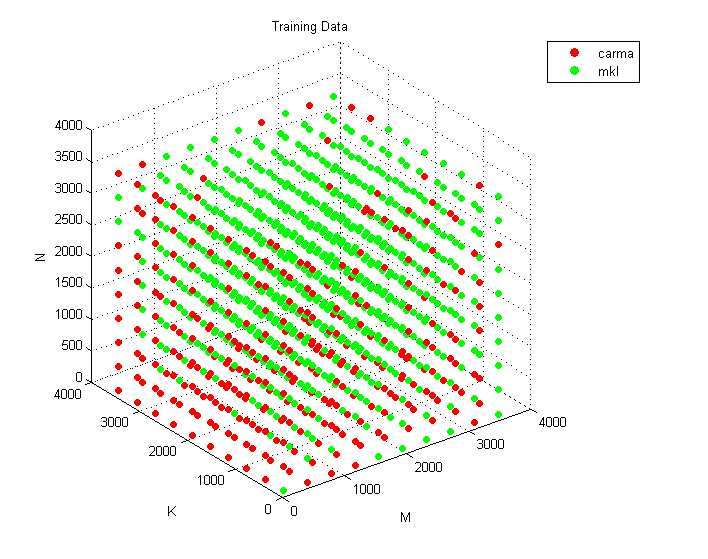
\includegraphics[width=\textwidth]{figures/emerald_train.png}
            \caption{Emerald}
            \label{f:train_emerald}
            \end{subfigure}
        \begin{subfigure}[t]{0.3\textwidth}
            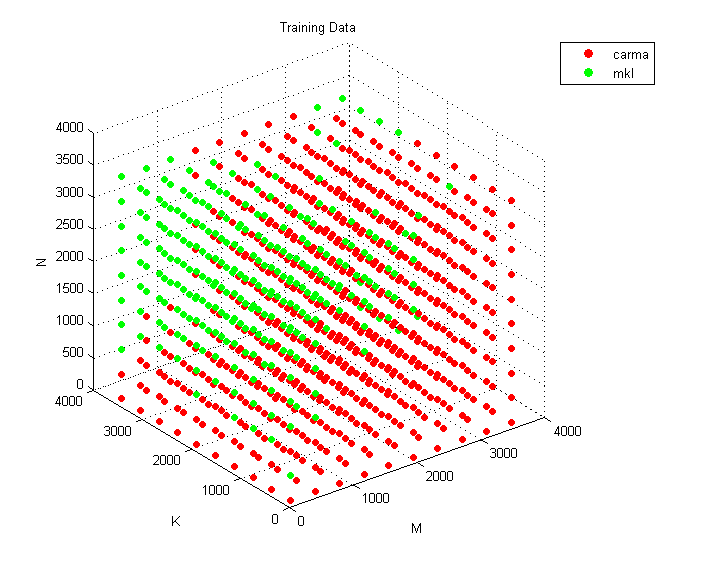
\includegraphics[width=\textwidth]{figures/hopper_train.png}
            \caption{Hopper}
            \label{f:train_hopper}
        \end{subfigure}
        \begin{subfigure}[t]{0.3\textwidth}
            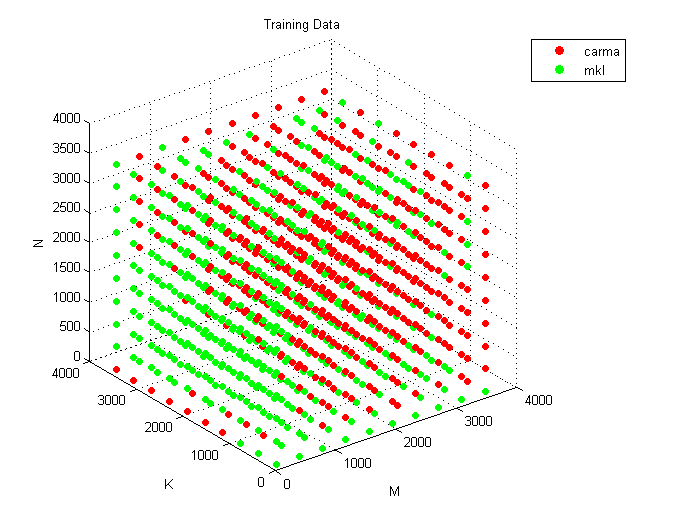
\includegraphics[width=\textwidth]{figures/sandy_train.png}
            \caption{Sandy}
            \label{f:train_sandy}
        \end{subfigure}
        \caption{Training results for each of our three machines. Green dots represent data points where MKL outperformed CARMA, red dots indicate the reverse. Note how the results are almost completely reversed for Emerald and Sandy.}
    \label{fig:training}
\end{figure*}

Another surprising result of our training was the fact that CARMA performed well for such large regions.
The developers of that algorithm had designed it for multiplication of ``long, skinny'' matrices, and it outperformed MKL for those on all three of our machines.
However, its strong performance for other types of matrices was unexpected.
This is likely to do with... \shaddi{something?}.

\subsection{Classification Performance}
